% Options for packages loaded elsewhere
% Options for packages loaded elsewhere
\PassOptionsToPackage{unicode}{hyperref}
\PassOptionsToPackage{hyphens}{url}
\PassOptionsToPackage{dvipsnames,svgnames,x11names}{xcolor}
%
\documentclass[
  11pt,
]{article}
\usepackage{xcolor}
\usepackage{amsmath,amssymb}
\setcounter{secnumdepth}{5}
\usepackage{iftex}
\ifPDFTeX
  \usepackage[T1]{fontenc}
  \usepackage[utf8]{inputenc}
  \usepackage{textcomp} % provide euro and other symbols
\else % if luatex or xetex
  \usepackage{unicode-math} % this also loads fontspec
  \defaultfontfeatures{Scale=MatchLowercase}
  \defaultfontfeatures[\rmfamily]{Ligatures=TeX,Scale=1}
\fi
\usepackage{lmodern}
\ifPDFTeX\else
  % xetex/luatex font selection
\fi
% Use upquote if available, for straight quotes in verbatim environments
\IfFileExists{upquote.sty}{\usepackage{upquote}}{}
\IfFileExists{microtype.sty}{% use microtype if available
  \usepackage[]{microtype}
  \UseMicrotypeSet[protrusion]{basicmath} % disable protrusion for tt fonts
}{}
\usepackage{setspace}
\makeatletter
\@ifundefined{KOMAClassName}{% if non-KOMA class
  \IfFileExists{parskip.sty}{%
    \usepackage{parskip}
  }{% else
    \setlength{\parindent}{0pt}
    \setlength{\parskip}{6pt plus 2pt minus 1pt}}
}{% if KOMA class
  \KOMAoptions{parskip=half}}
\makeatother
% Make \paragraph and \subparagraph free-standing
\makeatletter
\ifx\paragraph\undefined\else
  \let\oldparagraph\paragraph
  \renewcommand{\paragraph}{
    \@ifstar
      \xxxParagraphStar
      \xxxParagraphNoStar
  }
  \newcommand{\xxxParagraphStar}[1]{\oldparagraph*{#1}\mbox{}}
  \newcommand{\xxxParagraphNoStar}[1]{\oldparagraph{#1}\mbox{}}
\fi
\ifx\subparagraph\undefined\else
  \let\oldsubparagraph\subparagraph
  \renewcommand{\subparagraph}{
    \@ifstar
      \xxxSubParagraphStar
      \xxxSubParagraphNoStar
  }
  \newcommand{\xxxSubParagraphStar}[1]{\oldsubparagraph*{#1}\mbox{}}
  \newcommand{\xxxSubParagraphNoStar}[1]{\oldsubparagraph{#1}\mbox{}}
\fi
\makeatother


\usepackage{longtable,booktabs,array}
\usepackage{calc} % for calculating minipage widths
% Correct order of tables after \paragraph or \subparagraph
\usepackage{etoolbox}
\makeatletter
\patchcmd\longtable{\par}{\if@noskipsec\mbox{}\fi\par}{}{}
\makeatother
% Allow footnotes in longtable head/foot
\IfFileExists{footnotehyper.sty}{\usepackage{footnotehyper}}{\usepackage{footnote}}
\makesavenoteenv{longtable}
\usepackage{graphicx}
\makeatletter
\newsavebox\pandoc@box
\newcommand*\pandocbounded[1]{% scales image to fit in text height/width
  \sbox\pandoc@box{#1}%
  \Gscale@div\@tempa{\textheight}{\dimexpr\ht\pandoc@box+\dp\pandoc@box\relax}%
  \Gscale@div\@tempb{\linewidth}{\wd\pandoc@box}%
  \ifdim\@tempb\p@<\@tempa\p@\let\@tempa\@tempb\fi% select the smaller of both
  \ifdim\@tempa\p@<\p@\scalebox{\@tempa}{\usebox\pandoc@box}%
  \else\usebox{\pandoc@box}%
  \fi%
}
% Set default figure placement to htbp
\def\fps@figure{htbp}
\makeatother





\setlength{\emergencystretch}{3em} % prevent overfull lines

\providecommand{\tightlist}{%
  \setlength{\itemsep}{0pt}\setlength{\parskip}{0pt}}



 


\makeatletter
\@ifpackageloaded{caption}{}{\usepackage{caption}}
\AtBeginDocument{%
\ifdefined\contentsname
  \renewcommand*\contentsname{Table of contents}
\else
  \newcommand\contentsname{Table of contents}
\fi
\ifdefined\listfigurename
  \renewcommand*\listfigurename{List of Figures}
\else
  \newcommand\listfigurename{List of Figures}
\fi
\ifdefined\listtablename
  \renewcommand*\listtablename{List of Tables}
\else
  \newcommand\listtablename{List of Tables}
\fi
\ifdefined\figurename
  \renewcommand*\figurename{Figure}
\else
  \newcommand\figurename{Figure}
\fi
\ifdefined\tablename
  \renewcommand*\tablename{Table}
\else
  \newcommand\tablename{Table}
\fi
}
\@ifpackageloaded{float}{}{\usepackage{float}}
\floatstyle{ruled}
\@ifundefined{c@chapter}{\newfloat{codelisting}{h}{lop}}{\newfloat{codelisting}{h}{lop}[chapter]}
\floatname{codelisting}{Listing}
\newcommand*\listoflistings{\listof{codelisting}{List of Listings}}
\makeatother
\makeatletter
\makeatother
\makeatletter
\@ifpackageloaded{caption}{}{\usepackage{caption}}
\@ifpackageloaded{subcaption}{}{\usepackage{subcaption}}
\makeatother
\usepackage{bookmark}
\IfFileExists{xurl.sty}{\usepackage{xurl}}{} % add URL line breaks if available
\urlstyle{same}
\hypersetup{
  pdftitle={Heat transfer across concrete cracks: quantifying thermal resistance using Abaqus},
  pdfauthor={Jinpeng Zhu},
  colorlinks=true,
  linkcolor={blue},
  filecolor={Maroon},
  citecolor={Blue},
  urlcolor={Blue},
  pdfcreator={LaTeX via pandoc}}


% UofA Engineering Assignment Title Page Partial
% This partial customizes the title page for University of Alberta engineering assignments

% Page geometry and spacing
% \setlength{\textwidth}{6.5in}
% \setlength{\textheight}{9.in}
% \setlength{\oddsidemargin}{0in}
% \setlength{\headheight}{0in}

\usepackage[margin=3cm]{geometry}
\makeatletter
\makeatother


% Custom title page for UofA Engineering Assignment
\renewcommand\maketitle{
    \begin{flushleft}
        Student Name: Jinpeng Zhu \\
        Student ID: 1907843
        
    \end{flushleft}

    \begin{flushright}\vspace{-15mm}
        
\includegraphics[height=2cm]{../../Assets/template/uofa-eng-assignment-partial/logo.png}
    \end{flushright}

    \begin{center}\vspace{-1cm}
        \textbf{\large Proposal for Term Paper (CIV-E-665)}\\
        Heat transfer across concrete cracks: quantifying thermal
resistance using Abaqus
    \end{center}

    \rule{\linewidth}{0.1mm}

    \bigskip
    \bigskip
}
\begin{document}
\maketitle


\setstretch{1.4}
\section{Background and Motivation}\label{background-and-motivation}

Cracking is common in concrete due to shrinkage, loading, and thermal
cycling, and it can significantly affect heat transfer in addition to
durability and strength, as shown in the Figure~\ref{fig-fracture-demo}.
In underground structures, cold-region infrastructure, thermal
protection systems, and subsurface energy applications, cracks influence
serviceability, operational safety, and long-term performance.

\begin{figure}[H]

\centering{

\pandocbounded{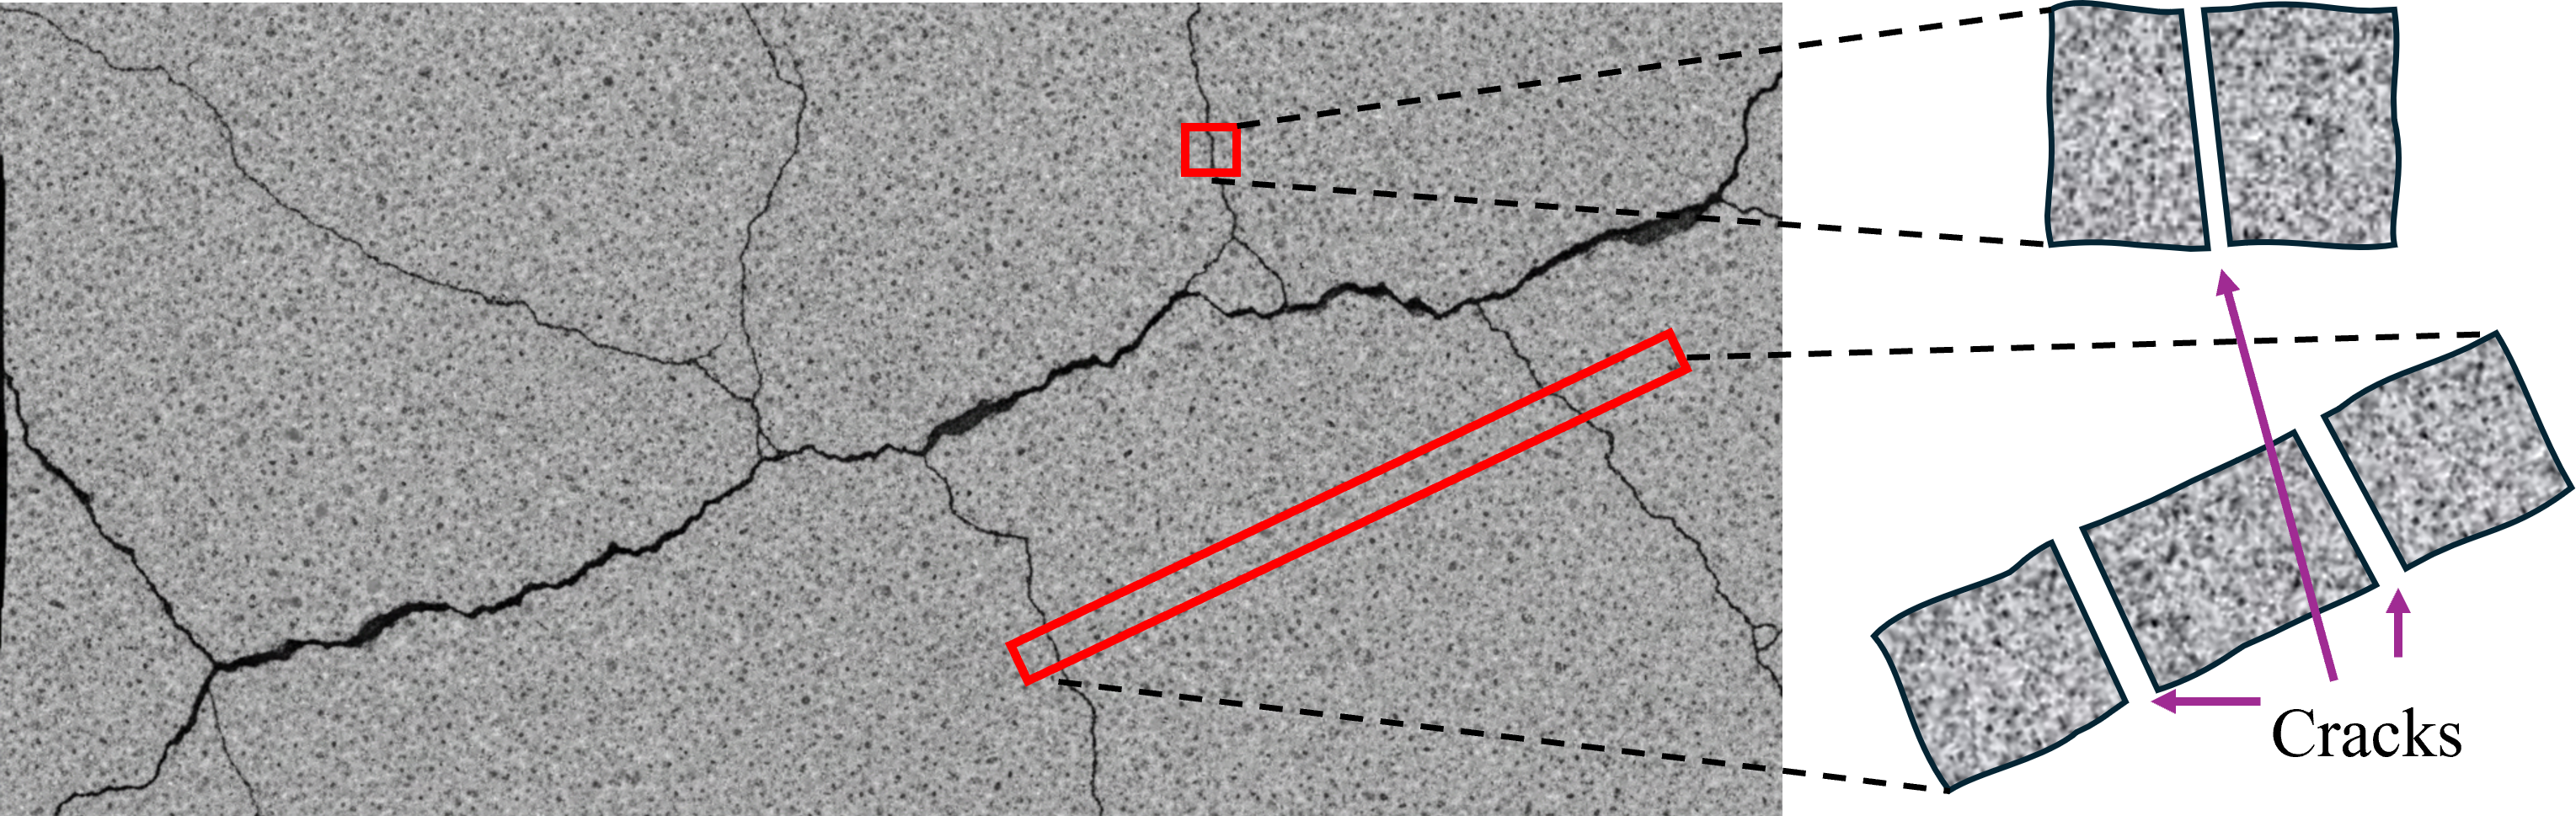
\includegraphics[keepaspectratio]{./assests/fractures_demo.png}}

}

\caption{\label{fig-fracture-demo}The illustration of concrete cracks,
which are simplified as a straight line in microperspective view in
order to facilitate the exploration of its impact}

\end{figure}%

A crack interrupts solid conduction and forces heat to cross a gap (air,
moisture, or infill), and in some cases radiation also contributes. This
can produce a temperature change at the crack and reduce the effective
thermal conductivity of the member. The magnitude of this thermal
barrier depends mainly on the crack aperture \(d\) (clearance) and the
crack geometry, particularly whether the crack is planar or tortuous
(which increases effective path length in 2D or interface area in 3D).

Most existing approaches represent cracking through homogenized
effective properties, but the thermal effect of a small number of
controlled cracks is less directly quantified in a way that can be
verified. This term paper will develop and verify an Abaqus-based FEM
workflow to quantify heat transfer across cracked concrete, focusing on
how crack aperture and crack geometry (planar versus tortuous) control
the equivalent interface thermal resistance under prescribed thermal
loading, while also using the project to build practical understanding
of FEM modeling and how to apply it to real engineering problems.
Assuming isotropic concrete to make sure the interpretation and
validation possible.

\section{Methods}\label{methods}

This study combines finite element modeling in Abaqus with simplified
analytical checks to quantify crack-controlled thermal resistance in
concrete. The properties of concrete and air are easy to get from
previous literature or industry database.

\textbf{Finite element simulation (Abaqus)}: The numerical work is
organized into three geometry stages (see Figure~\ref{fig-geometry}): 1)
single planar crack with uniform aperture \(d\); 2) two planar cracks
(two interfaces) each with aperture \(d\); 3) single tortuous crack with
the same nominal aperture \(d\), but a longer crack path (2D) or larger
effective interface area (3D). Thermal loading will be applied as
prescribed temperatures \(T_h\) and \(T_c\) on opposite boundaries to
create a steady temperature gradient and an approximately 1D heat-flow
direction in the far field. Mechanical loading will be neglected to keep
verification clean; crack aperture \(d\) will be prescribed
geometrically rather than computed from a coupled stress analysis.

\begin{figure}[H]

\centering{

\pandocbounded{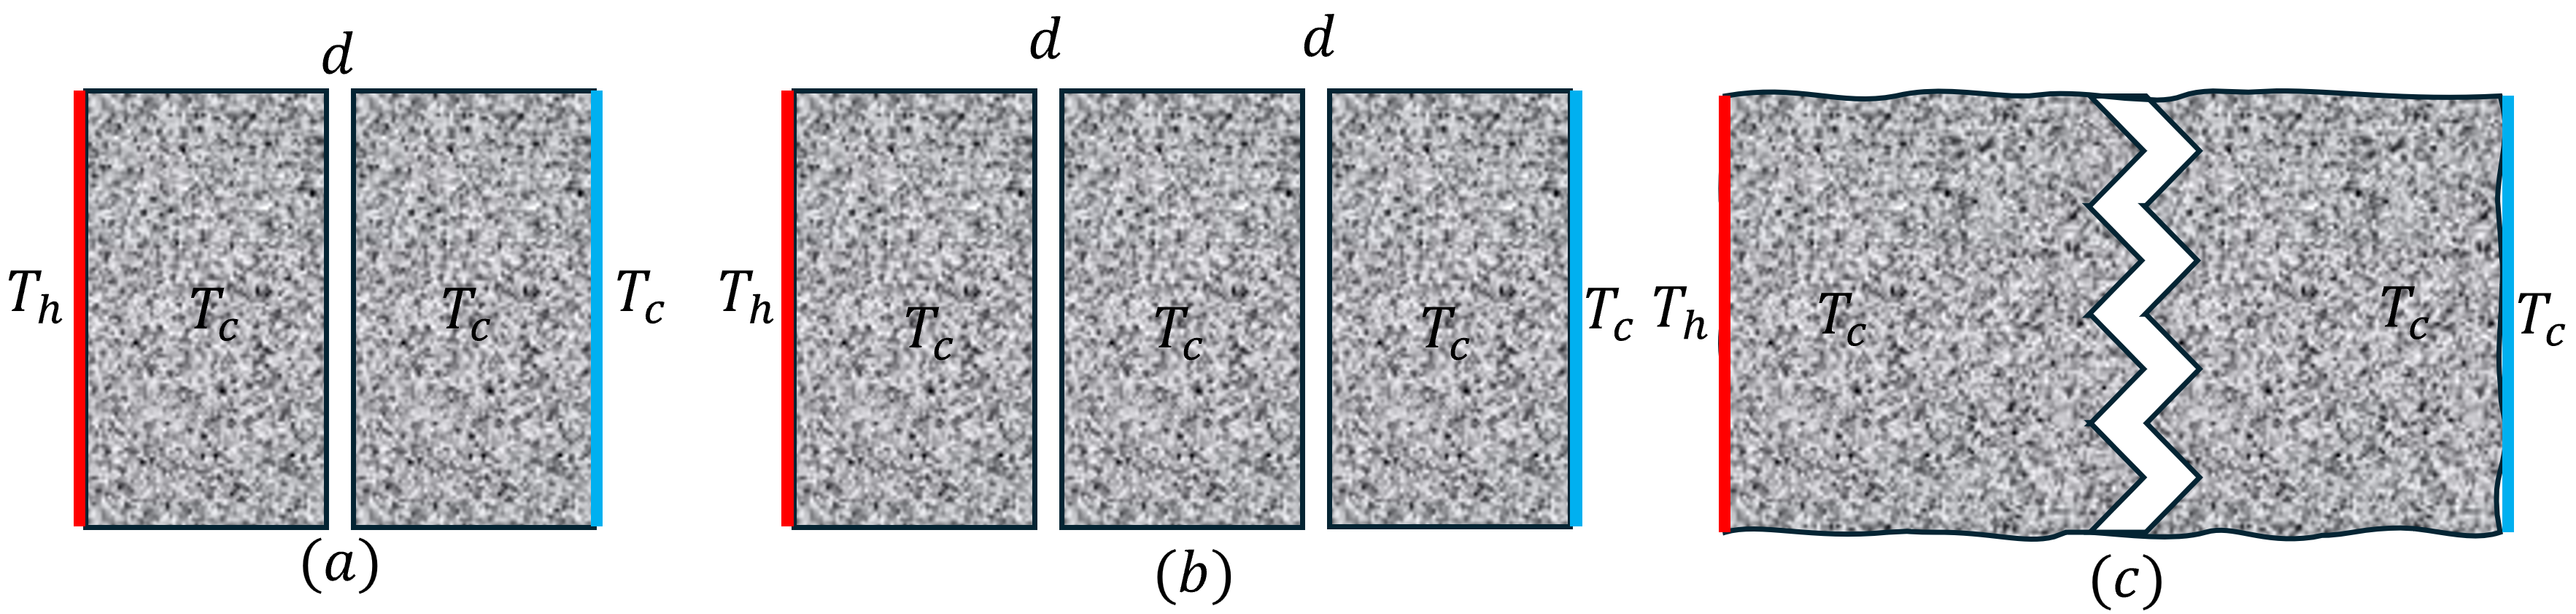
\includegraphics[keepaspectratio]{./assests/geometry_setting.png}}

}

\caption{\label{fig-geometry}The tentative geometry setting}

\end{figure}%

\textbf{Analytical verification}: Form Abaqus outputs, an equivalent
area-specific interface resistance. For verification and applying the
FEM knowledge from the class, another results from hand-verifying will
be compared and discussed with the Abaqus outputs.

\section{Tentative Timeline}\label{tentative-timeline}

\begin{longtable}[]{@{}
  >{\raggedright\arraybackslash}p{(\linewidth - 4\tabcolsep) * \real{0.0556}}
  >{\raggedright\arraybackslash}p{(\linewidth - 4\tabcolsep) * \real{0.1111}}
  >{\raggedright\arraybackslash}p{(\linewidth - 4\tabcolsep) * \real{0.8333}}@{}}
\toprule\noalign{}
\begin{minipage}[b]{\linewidth}\raggedright
Week
\end{minipage} & \begin{minipage}[b]{\linewidth}\raggedright
Due Date
\end{minipage} & \begin{minipage}[b]{\linewidth}\raggedright
Main work
\end{minipage} \\
\midrule\noalign{}
\endhead
\bottomrule\noalign{}
\endlastfoot
9 & Mar 03 & learning Abaqus \\
10 & Mar 10 & literature review \\
11 & Mar 17 & modeling \\
12 & Mar 24 & hand verification \\
13 & Mar 31 & organize and analysis results, draft manuscript \\
14 & Apr 07 & revise, finalize, and submit \\
\end{longtable}




\end{document}
